\documentclass[border=3mm]{standalone}
\usepackage[utf8]{inputenc}
\usepackage{tikz}
\usepackage{amsmath}
\usepackage[scaled=0.95]{helvet}
\renewcommand{\familydefault}{\sfdefault}

\begin{document}
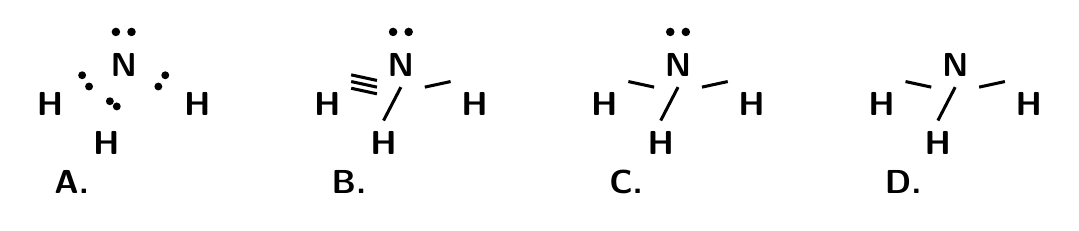
\begin{tikzpicture}[font=\sffamily\bfseries\large, line width=1.1pt, xscale=1.1, yscale=1.1]

% --- OPTION A ---
\begin{scope}[shift={(0,0)}]
    \node (Na) at (0,0) {N};
    \node (H1a) at (-0.85,-0.45) {H};
    \node (H2a) at (-0.2,-0.9) {H};
    \node (H3a) at (0.85,-0.45) {H};
    % dots on top
    \fill (-0.09, 0.38) circle (1.4pt);
    \fill (0.09, 0.38) circle (1.4pt);
    % dots between N and H1
    \fill (-0.48, -0.12) circle (1.3pt);
    \fill (-0.40, -0.25) circle (1.3pt);
    % dots between N and H2
    \fill (-0.16, -0.42) circle (1.3pt);
    \fill (-0.08, -0.48) circle (1.3pt);
    % dots between N and H3
    \fill (0.48, -0.12) circle (1.3pt);
    \fill (0.40, -0.25) circle (1.3pt);
    \node at (-0.6, -1.35) {\textbf{A.}};
\end{scope}

% --- OPTION B ---
\begin{scope}[shift={(3.2,0)}]
    \node (Nb) at (0,0) {N};
    \node (H1b) at (-0.85,-0.45) {H};
    \node (H2b) at (-0.2,-0.9) {H};
    \node (H3b) at (0.85,-0.45) {H};
    % dots on top
    \fill (-0.09, 0.38) circle (1.4pt);
    \fill (0.09, 0.38) circle (1.4pt);
    % triple bond between N and H1
    \draw ([yshift=2.2pt]Nb.south west) -- ([yshift=2.2pt]H1b.north east);
    \draw (Nb.south west) -- (H1b.north east);
    \draw ([yshift=-2.2pt]Nb.south west) -- ([yshift=-2.2pt]H1b.north east);
    % single bond N-H2
    \draw (Nb.south) -- (H2b.north);
    % single bond N-H3
    \draw (Nb.south east) -- (H3b.north west);
    \node at (-0.6, -1.35) {\textbf{B.}};
\end{scope}

% --- OPTION C ---
\begin{scope}[shift={(6.4,0)}]
    \node (Nc) at (0,0) {N};
    \node (H1c) at (-0.85,-0.45) {H};
    \node (H2c) at (-0.2,-0.9) {H};
    \node (H3c) at (0.85,-0.45) {H};
    % dots on top
    \fill (-0.09, 0.38) circle (1.4pt);
    \fill (0.09, 0.38) circle (1.4pt);
    % single bonds
    \draw (Nc.south west) -- (H1c.north east);
    \draw (Nc.south) -- (H2c.north);
    \draw (Nc.south east) -- (H3c.north west);
    \node at (-0.6, -1.35) {\textbf{C.}};
\end{scope}

% --- OPTION D ---
\begin{scope}[shift={(9.6,0)}]
    \node (Nd) at (0,0) {N};
    \node (H1d) at (-0.85,-0.45) {H};
    \node (H2d) at (-0.2,-0.9) {H};
    \node (H3d) at (0.85,-0.45) {H};
    % single bonds (no dots)
    \draw (Nd.south west) -- (H1d.north east);
    \draw (Nd.south) -- (H2d.north);
    \draw (Nd.south east) -- (H3d.north west);
    \node at (-0.6, -1.35) {\textbf{D.}};
\end{scope}

\end{tikzpicture}
\end{document}
